\documentclass[oneside, 11pt]{article}

\usepackage[T1]{fontenc}
\usepackage[utf8]{inputenc}
\usepackage[dutch]{babel}

\usepackage{fouriernc}
\usepackage[detect-all, load-configurations=binary,
            separate-uncertainty=true, per-mode=symbol,
            retain-explicit-plus, range-phrase={ tot }]{siunitx}

\usepackage{setspace}
\setstretch{1.2}

\setlength{\parskip}{\smallskipamount}
\setlength{\parindent}{0pt}

\usepackage{geometry}
\geometry{marginparwidth=0.5cm, verbose, a4paper, tmargin=3cm, bmargin=3cm, lmargin=2cm, rmargin=2cm}

\usepackage{float}

\usepackage[fleqn]{amsmath}
\numberwithin{equation}{section}
\numberwithin{figure}{section}

\usepackage{graphicx}
\graphicspath{{Figures/}}
\usepackage{subfig}

\usepackage{tikz}
\usetikzlibrary{plotmarks}

\usepackage{fancyhdr}
\pagestyle{fancy}
\fancyhf{}
\rhead{\thepage}
\renewcommand{\footrulewidth}{0pt}
\renewcommand{\headrulewidth}{0pt}

\usepackage{relsize}
\usepackage{xspace}
\usepackage{url}

\newcommand{\figref}[1]{Figuur~\ref{#1}}

\newcommand{\hisparc}{\textsmaller{HiSPARC}\xspace}
\newcommand{\kascade}{\textsmaller{KASCADE}\xspace}
\newcommand{\sapphire}{\textsmaller{SAPPHiRE}\xspace}
\newcommand{\jsparc}{\textsmaller{jSparc}\xspace}
\newcommand{\hdf}{\textsmaller{HDF5}\xspace}
\newcommand{\aires}{\textsmaller{AIRES}\xspace}
\newcommand{\csv}{\textsmaller{CSV}\xspace}
\newcommand{\python}{\textsmaller{PYTHON}\xspace}
\newcommand{\corsika}{\textsmaller{CORSIKA}\xspace}
\newcommand{\labview}{\textsmaller{LabVIEW}\xspace}
\newcommand{\daq}{\textsmaller{DAQ}\xspace}
\newcommand{\adc}{\textsmaller{ADC}\xspace}
\newcommand{\adcs}{\textsmaller{ADC}s\xspace}
\newcommand{\Adcs}{A\textsmaller{DC}s\xspace}
\newcommand{\hi}{\textsc{h i}\xspace}
\newcommand{\hii}{\textsc{h ii}\xspace}
\newcommand{\mip}{\textsmaller{MIP}\xspace}
\newcommand{\hisparcii}{\textsmaller{HiSPARC II}\xspace}
\newcommand{\hisparciii}{\textsmaller{HiSPARC III}\xspace}
\newcommand{\pmt}{\textsmaller{PMT}\xspace}
\newcommand{\pmts}{\textsmaller{PMT}s\xspace}

\DeclareSIUnit{\electronvolt}{\ensuremath{\mathrm{e\!\!\:V}}}

\DeclareSIUnit{\unitsigma}{\ensuremath{\sigma}}
\DeclareSIUnit{\mip}{\textsmaller{MIP}}
\DeclareSIUnit{\adc}{\textsmaller{ADC}}

\DeclareSIUnit{\gauss}{G}
\DeclareSIUnit{\parsec}{pc}
\DeclareSIUnit{\year}{yr}



\begin{document}

\title{Dagelijkse controle van een station} \author{C.G.N. van Veen}
\date{}

\maketitle

\section{Stations}

\hisparc heeft verschillende meetstations op scholen in heel Nederland
staan. De stations meten onophoudelijk en verzenden hun data naar de \hisparc database. 
De status van de \hisparc stations wordt bijgehouden door Nagios. 
Informatie over de status van een station is te vinden op \url{http://data.hisparc.nl}. 
Dit document geeft aan hoe de status van een station optimaal gemaakt kan worden.

\section{Status van een station controleren}

De school of instelling is verantwoordelijk voor het onderhoud van het meetstation. 
Op de site: \url{http://data.hisparc.nl} kunnen de prestaties van het station worden gevolgd. Van deze site is in figuur
\ref{fig:frontweb} een screenshot te zien is. Op de site staan alle
stations vermeld die in het netwerk van \hisparc zijn aangesloten. De
cirkels voor de stations geven met een kleurcode aan wat de status van
een station is. Als de kleur van de cirkel voor het betreffende station
groen is, dan is de status van het station `in orde'. Een gele cirkel
geeft aan dat er een probleem is met het station. Rood betekent dat de pc
niet `gepingt' kan worden, vaak staat de pc dan uit, heeft de pc geen internet of VPN werkt niet.

\begin{figure} \centering 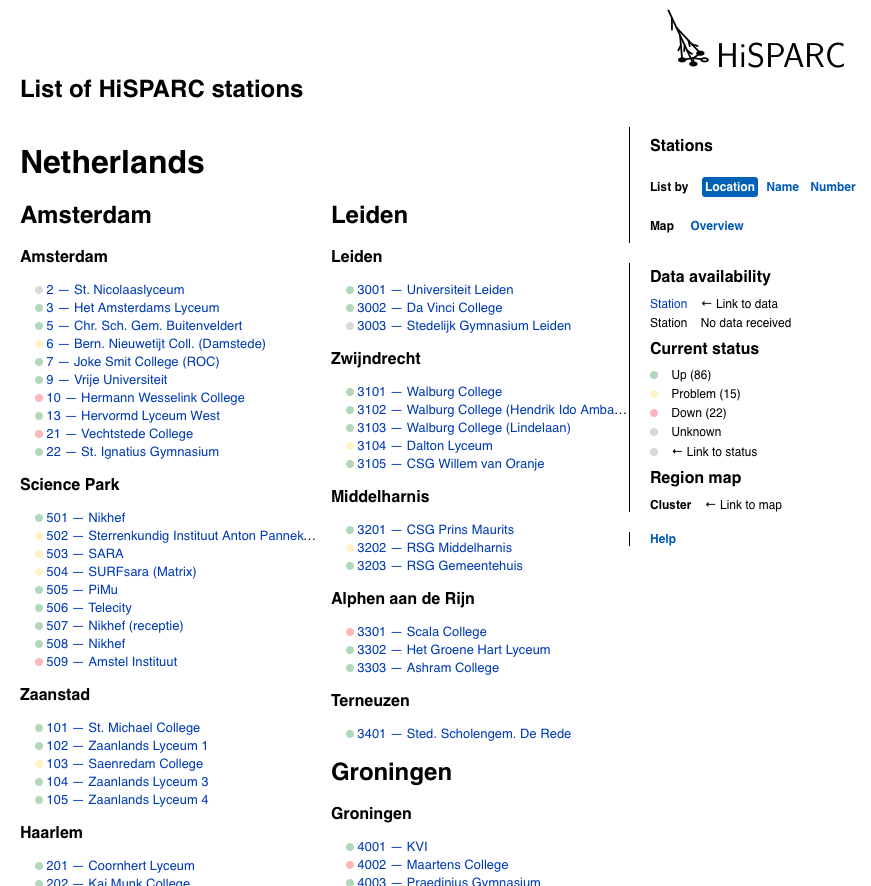
\includegraphics[scale=0.60]{websitefront}
\caption{Screenshot van de \hisparc data website.} 
\label{fig:frontweb}
\end{figure}

\section{Probleem met een station}

In het geval van een gele of rode cirkel, kunt u klikken op de link van het
desbetreffende station (bijvoorbeeld klikken op: \underline{501-Nikhef}) zoals te zien is in figuur \ref{fig:frontweb}. 
Dan wordt u doorgelinkt naar de status pagina van het betreffende station. Zo'n
pagina met een overzicht van verzonden data van een eerdere dagen
van een station is weergeven in figuur \ref{fig:websiteerror}. In figuur \ref{fig:websiteerror}
is te zien dat het station niet meer meet na 14.00 uur op de vorige dag,  omdat het aantal
gemeten events naar nul gaat. In het Pulseheight histogram is ook te zien
dat de \mip piek niet goed aanwezig is, wat duidt op een verkeerde
instelling van de \pmt. Zie ook \cite{inregelen}.

\begin{figure} 
\centering 
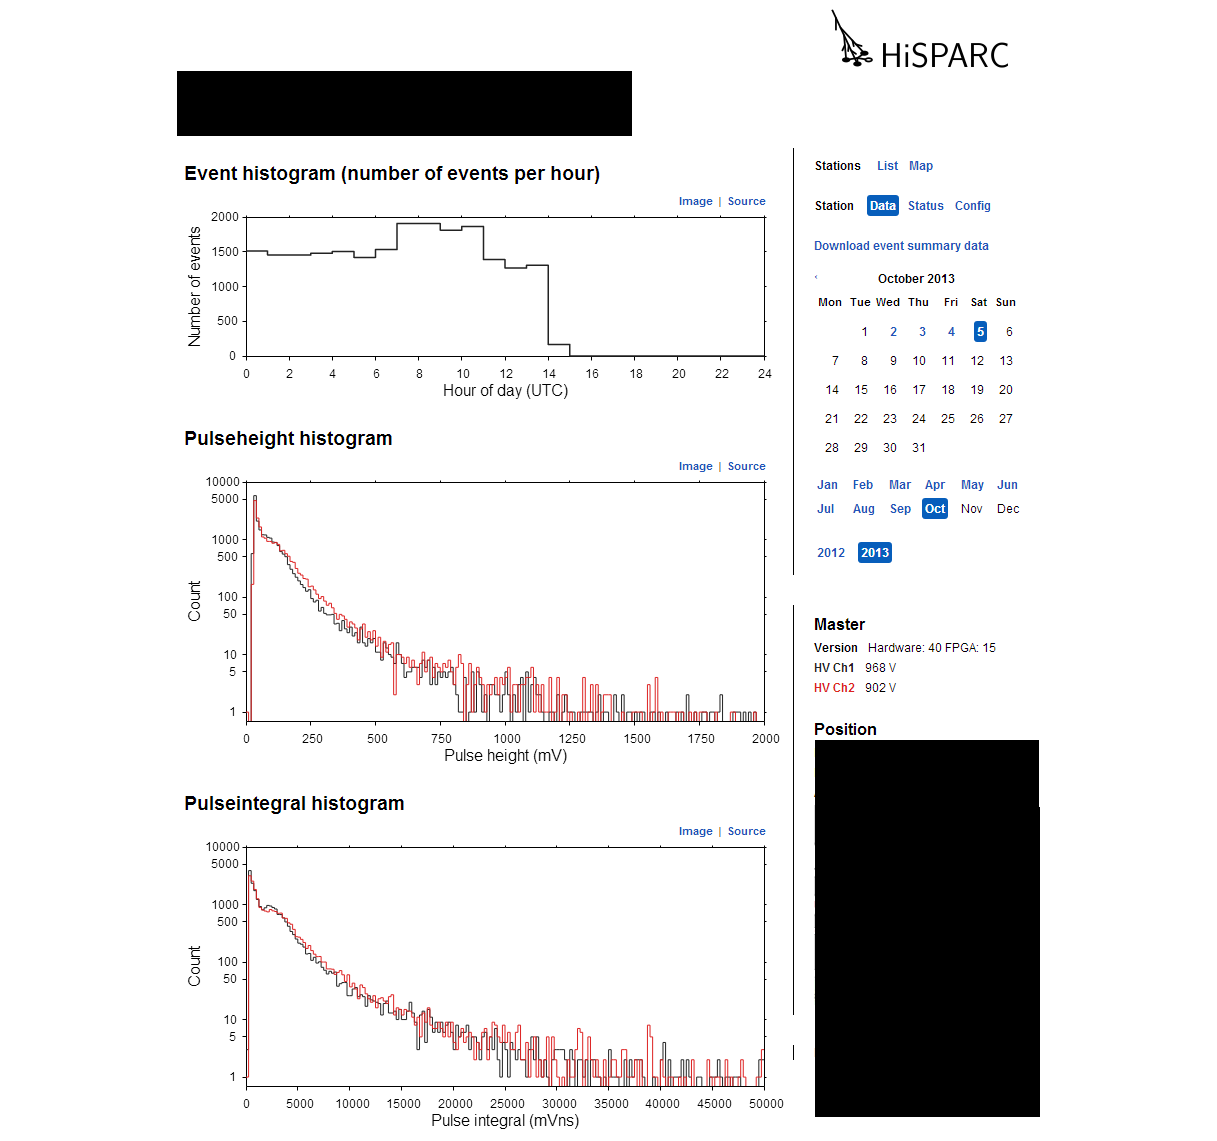
\includegraphics[scale=0.40]{websiteerror}
\caption{Screenshot van het data-overzicht van een
station. In het event histogram is duidelijk te zien dat het station
niets meer heeft gemeten na 14.00 uur UTC tijd. Ook is er in het pulseheight histogram
geen duidelijke MIP piek te zien.} \label{fig:websiteerror} 
\end{figure}

\section{Problemen oplossen}

Om precies te zien wat er mis is met het station en het probleem
daadwerkelijk op te lossen, klikt u op de site: \url{http://data.hisparc.nl} op het gekleurde cirkeltje voor het betreffende station. Als u op de status pagina zit kunt u op \emph{status} klikken rechtsboven op de status pagina van het station.
In beide gevallen krijgt u een status en problemen overzicht, zie figuur \ref{fig:statusstation}. 
In figuur \ref{fig:statusstation} is te zien dat de \emph{TriggerRate}
rood is en dus aandacht behoeft.
Om de problemen met de verschillende categorieën op te lossen is een speciale website ontwikkeld.
Ga naar \url{http://docs.hisparc.nl/maintenance/}, zie figuur \ref{fig:maintenance}. 
U kunt hier onder andere op \emph{known issues} klikken en op \emph{frequently asked questions}. 
Op de pagina \emph{known issues} bevindt zich een gecategoriseerde lijst van problemen. 
U kunt daar in de tweede alinea op het betreffende probleem klikken, voor het gegeven voorbeeld is dat \emph{TriggerRate}. 
Op de site verschijnt dan een lijst met problemen die een foutmelding \emph{TriggerRate} geven. 
In deze lijst is een oplossing te vinden voor het probleem, zie figuur \ref{fig:solution}.
Voor de foutmelding \emph{TriggerRate} vinden we dan als mogelijke oplossing dat de button \emph{DAQ Mode} moet worden gebruikt om van mode te wisselen.
Bij andere problemen met stations kunt u het bovenstaande stappenplan op dezelfde manier volgen om diverse storingen en problemen met u station op te lossen.
Komt u er alsnog niet uit neem dan contact op met de clustercoordinator of met \url{beheer@hisparc.nl}.
 

\begin{figure} 
\centering 
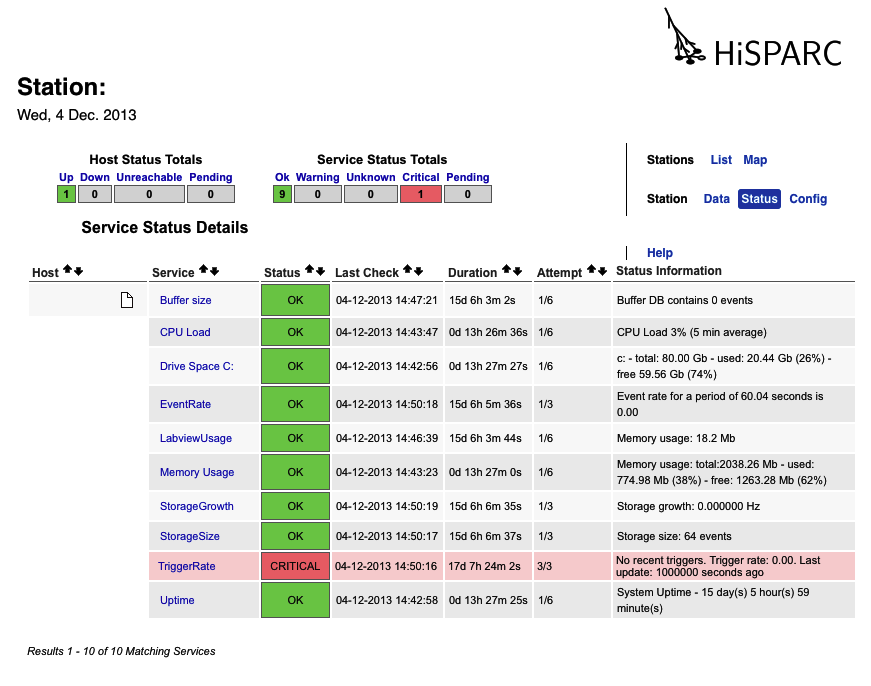
\includegraphics[scale=0.60]{statusstation}
\caption{Screenshot van de status van een station. In de tabel is in rood aangegeven 
welke foutmeldingen er voor het station zijn waargenomen. 
In dit geval is er een probleem met de \emph{TriggerRate}.}\label{fig:statusstation} 
\end{figure}

\begin{figure} 
\centering 
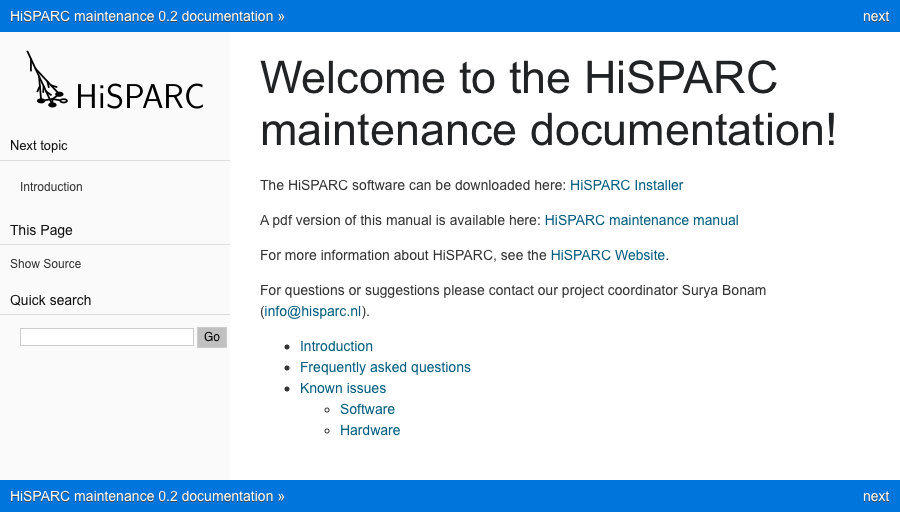
\includegraphics[scale=0.30]{maintenance}
\caption{Klik op \emph{frequently asked questions} en daarna op \emph{known issues} om naar verschillende foutmeldingen en oplossingen daarvan te gaan.}\label{fig:maintenance} 
\end{figure}
 
\begin{figure} 
\centering 
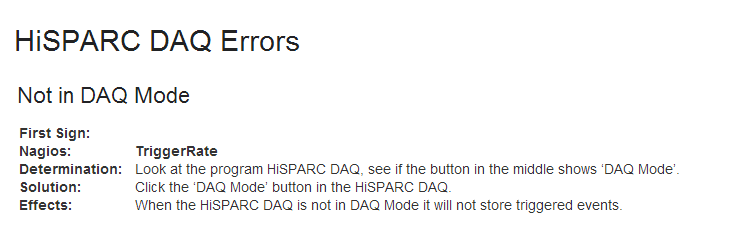
\includegraphics[scale=0.60]{solution}
\caption{Een mogelijke reden voor foutmelding en de bijhorende oplossing. Hier is de oplossing, om in het programma \hisparc DAQ op de button \emph{DAQ mode} te klikken.} 
\label{fig:solution} 
\end{figure}




\begin{thebibliography}{9} 
	
	\bibitem{inregelen} D.B.R.A. Fokkema, \emph{Inregelen PMT's}, infopakket \hisparc 
\end{thebibliography}



\end{document}
